\documentclass[12pt]{article}
\usepackage[spanish]{babel}

%%%%%%%%%%%%%%%%%%%%%%%%%%%%%%%%%%
%%%%%%%%%%%%%%%%%%%%%%%%%%%%%   %%
%%        Datos Trabajo     %%  %%
%%%%%%%%%%%%%%%%%%%%%%%%%%%%%%%%%%
\newcommand{\titulo}	[0]{Evidencia de aprendizaje: Problemáticas de su entorno}
\newcommand{\materia}	[0]{Desarrollo Sustentable}
\newcommand{\grupo}		[0]{BI-BDSU-2002-B1-012}
\newcommand{\unidad}	[0]{Unidad 2}


%%%%%%%%%%%%%%%%%%%%%%%%%%%%%%%%%%
%%%%%%%%%%%%%%%%%%%%%%%%%%%%%%%%%%
\usepackage{amssymb}
\usepackage{enumerate}
\usepackage{geometry}
\usepackage{mathtools}
\usepackage{multicol}
\usepackage{soul}

\usepackage{graphicx}
	\graphicspath{ {assets/} }

\usepackage{hyperref}
	\hypersetup{
			pdftex,
		        pdfauthor	={bench},
		        pdftitle	={\titulo},
		        pdfsubject	={\materia},
		        pdfkeywords	={\grupo, \unidad, UnADM},
		        pdfproducer	={Latex with hyperref, Ubuntu},
		        pdfcreator	={pdflatex},
			colorlinks	=true,
				linkcolor	=red,
				urlcolor	=cyan,
				filecolor	=yellow}

%%%%%%%%%%%%%%%%%%%%%%%%%%%%%%%%%%
%%%%%%%%%%%%%%%%%%%%%%%%%%%%%%%%%%

\title{
	
\includegraphics{../../../assets/logo-unadm} \\
	\ \\ Benjam\'in Rivera \\
	\bf{\titulo}\\\ \\}

\author{
	Universidad Abierta y a Distancia de México \\
	TSU en Biotecnolog\'ia \\
	\textit{Materia:} \materia \\
	\textit{Grupo:} \grupo \\
	\textit{Unidad:} \unidad \\
	\\
	\textit{Matricula:} ES202105994 }

\date{\textit{Fecha de entrega:} \today}


%%%%%%%%%%%%%%%%%%%%%%%%%%%%%
%%        Documento         %%
%%%%%%%%%%%%%%%%%%%%%%%%%%%%%%%
\begin{document}
\maketitle\newpage

	\begin{center}\par\bf\huge Contaminaci\'on de ladrilleras
	\end{center}
	
	\par Una actividad econ\'omica bastante popular en toda la rep\'ublica, es la producci\'on de ladrillos. Dicha actividad requiere, en ciera parte de su producci\'on, utilizar grandes fuentes de calor para poder \textit{cocer} el ladrillo y que convertir el maleable adobe en resistentes ladrillos. 

	\begin{figure}[h]
		\centering
		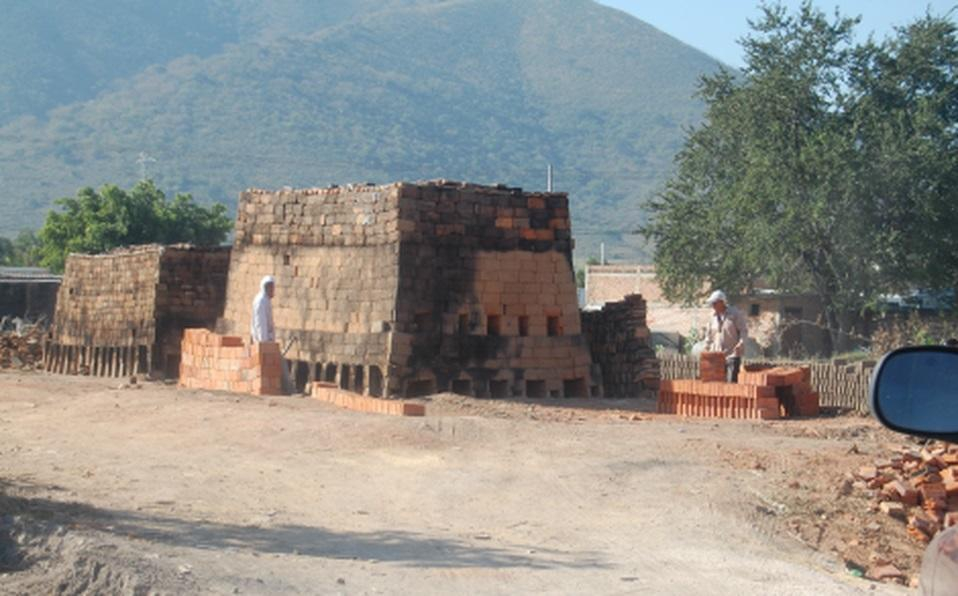
\includegraphics [width=0.49\textwidth] {quema_ladrillos.jpg}
		\caption{Horno de ladrillos.}
	\end{figure}

	\begin{figure}[h]
		\centering
		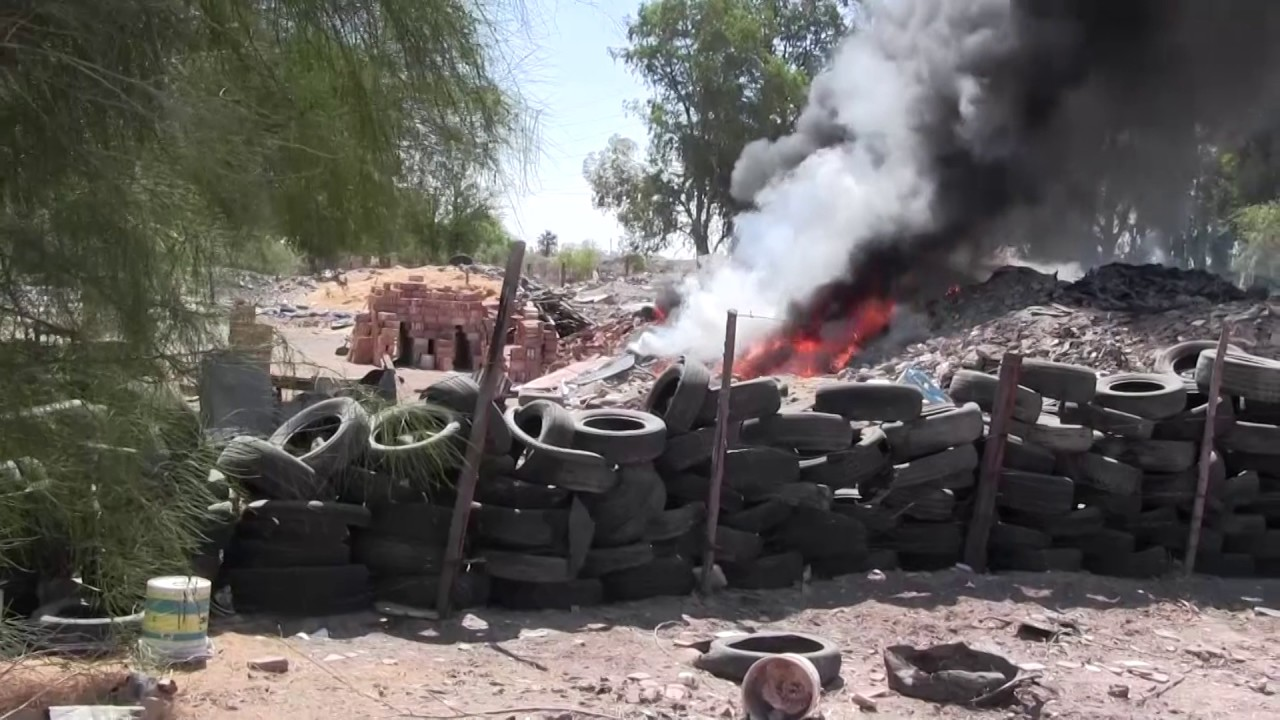
\includegraphics [width=0.49\textwidth] {fuego_ladrillos.jpg}
		\caption{Horno de ladrillos encendido y pilas de material utilizado en la combusti\'on.}
	\end{figure}


	\par Este es un tema complejo que crea varias problem\'aticas, las m\'as preocupantes son  

	\begin{quote}\begin{itemize}
		\item la contaminaci\'on del aire,
		\item la contaminaci\'on del agua, 
		\item el cambio clim\'atico y
		\item la perdida de biodiversidad.
	\end{itemize}\end{quote}
	se han evaluando diversas propuestas para combatir esta situación, entre ellas la reubicación, el cambio de combustible o producción de los ladrillos, sin embargo, el tema es complejo por la oposición de los involucrados.
	
	\par Al ser un problema tan complejo, y por desgracia tan com\'un en todo M\'exico, existen una infinidad de notas al respecto. La nota m\'as reciente que encontre fue \cite{noticia}, donde se explica la situaci\'on de esta problem\'atica \textbf{en la capital de \textit{San Luis Potosi}}.

	\begin{figure}[h]
		\centering
		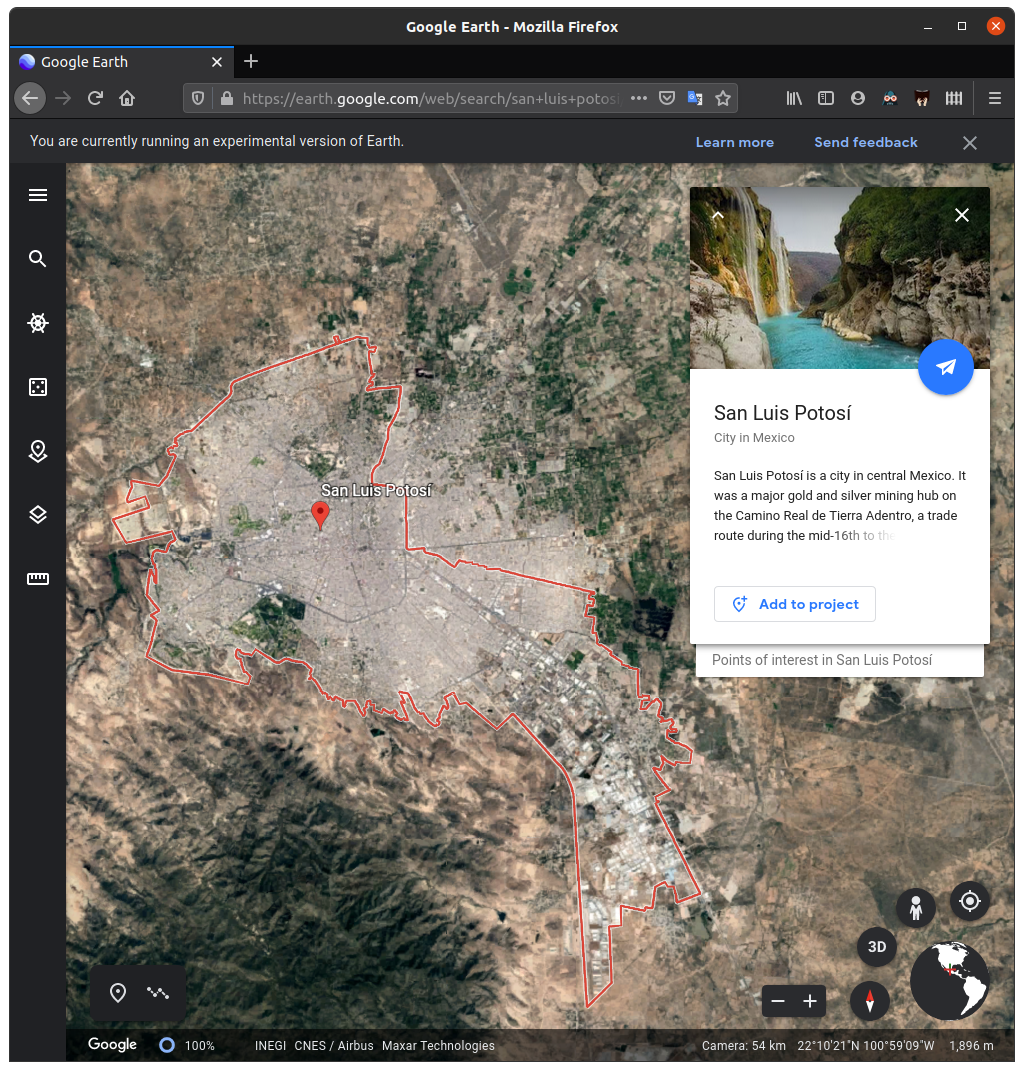
\includegraphics [width=0.6\textwidth] {San_Luis_Potosi-2.png}
		\caption{Imag\'en satelital de la localidad.}
	\end{figure}
	
	\par Desde el \textbf{ambito social} es necesario considerar la perspectiva de los productores y la comunidad. Los productores tienen tradiciones que les es dificil romper y pocos recursos para modernizarse; adem\'as no consideran los efectos negativos que pueden causar al resto de la comunidad. Por otro lado, la comunidad se queja inmediatamente de aumento en precios de ladrillos sin considerar lo que los productores deben hacer para adaptarse a las regulaciones y cuidar la salud de la comunidad.
	
	\par Respecto al \textbf{ambito econ\'omico}, los \'unicos realmente afectados son los productores, a quienes se les solicitan inversiones considerables para cambiar su fuente de combustible o para reubicarse en alguna zona de menor afectaci\'on ambiental y social.
	
	\par Y el \textbf{ambito ambiental} es el que m\'as esta sufriendo. El uso indebido de los combustoleos equivocados, y la liberaci\'on indiscriminada de gases al ambiente, han casusado muchos efectos negativos, como
	
	\begin{quote}\begin{itemize}
		\item enfermedades respiratorias en las comunidades cercanas,
		\item contaminaci\'on del agua,
		\item contaminaci\'on del aire y
		\item deforestaci\'on de zonas indebidas.
	\end{itemize}\end{quote}





\subsubsection*{Nota}
	\par La nota puede encontrarse en \cite{noticia}.
	
	\begin{figure}[h]
		\centering
		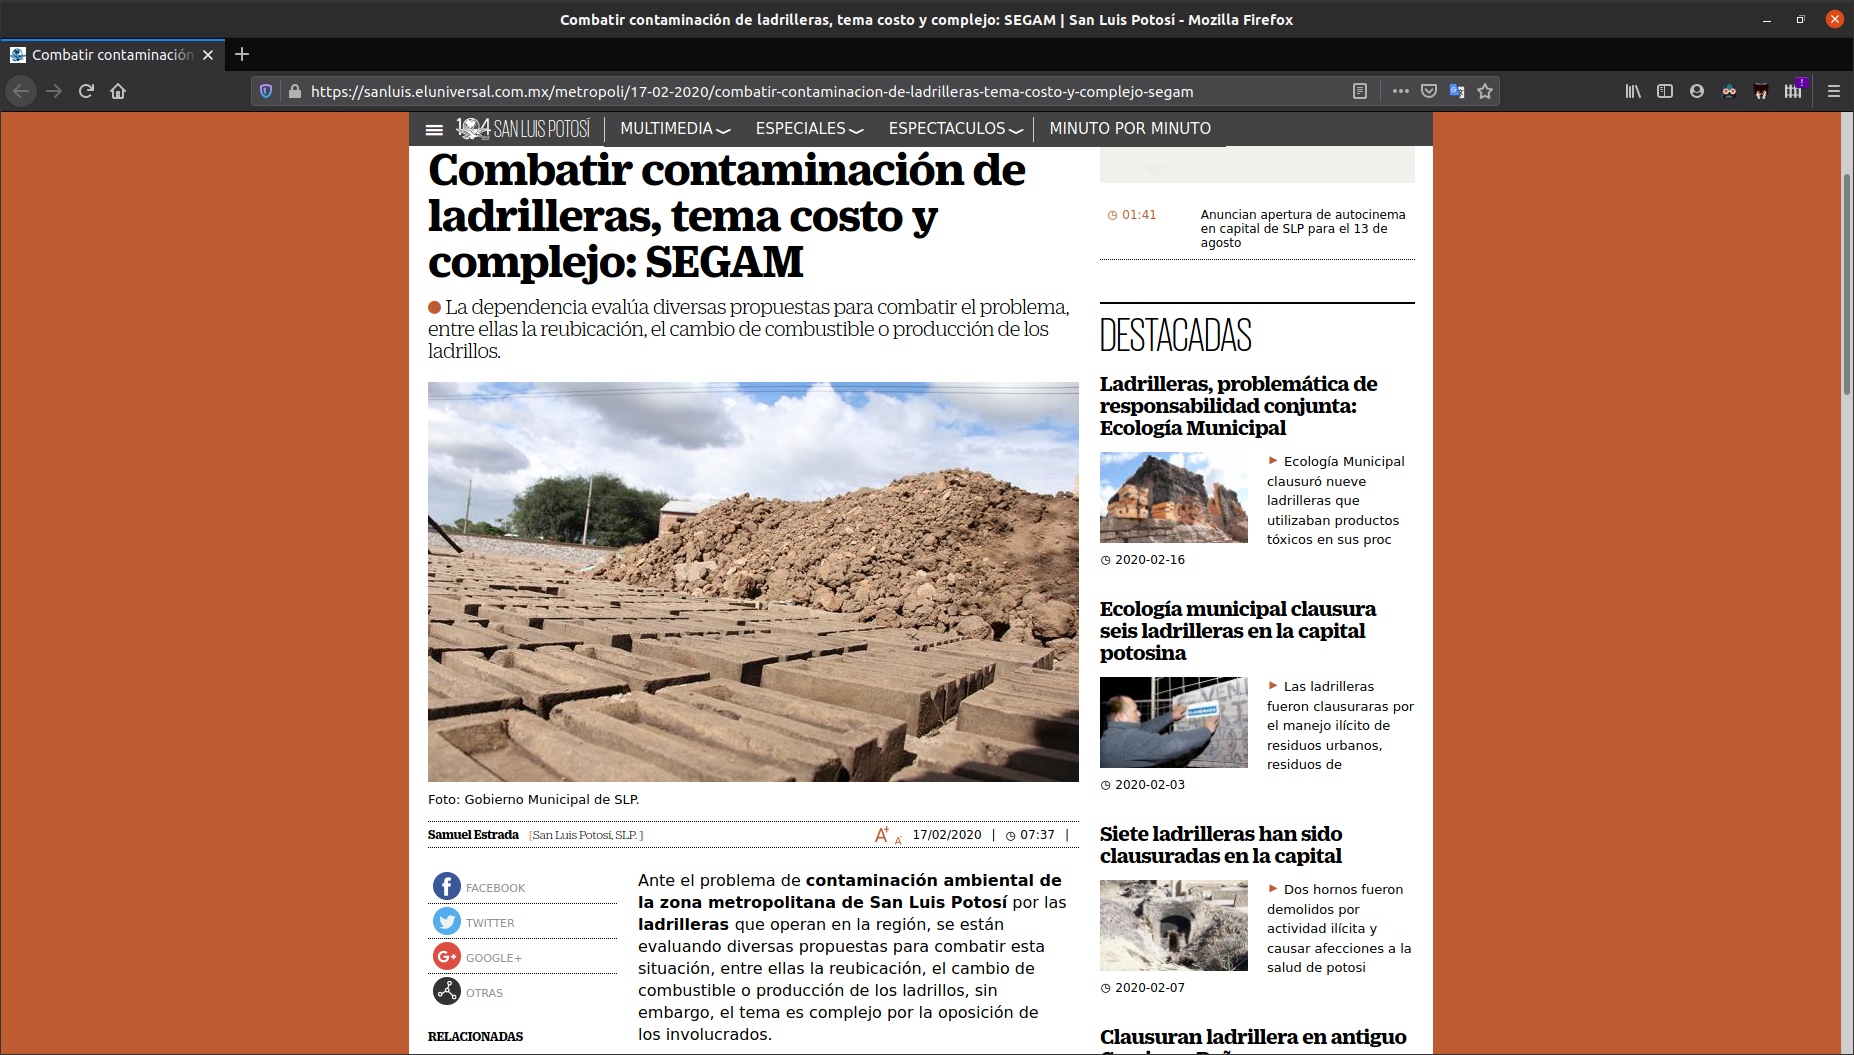
\includegraphics [width=0.6\textwidth] {nota-ladrillos-SLP.png}
		\caption{Captura de pantalla de la noticia.}
	\end{figure}

%%%%%%%%%%%%%%%%%%%%%%%%%%%%%%%%
%%         Bibliografia        %%
%%%%%%%%%%%%%%%%%%%%%%%%%%%%%%%%%%
\newpage
\begin{thebibliography}{X}
	
	\bibitem{basica} S/D. (2020). \textit{U2 $|$ Dimensiones y retos de la sustentabilidad}. \today, de UnADM. Sitio web: \url{https://dmd.unadmexico.mx/contenidos/DCSBA/BLOQUE1/BI/01/BDSU/unidad_02/descargables/BDSU_U2_Contenido.pdf} 
	
	\bibitem{noticia} Estrada, S.. (2020). \today{Combatir contaminación de ladrilleras, tema costo y complejo: SEGAM}. \today, de El Universal Sitio web: \url{https://sanluis.eluniversal.com.mx/metropoli/17-02-2020/combatir-contaminacion-de-ladrilleras-tema-costo-y-complejo-segam}
	
	\bibitem{ladrillos-visual} Edición. (2020). {\it Supera contaminación de ladrillos a administraciones}. \today, de Perdiodico Correo Sitio web: \url{https://periodicocorreo.com.mx/supera-contaminacion-de-ladrillos-a-administraciones/}
	\bibitem{enfermedades} Gallegos, A., Lang, B., Fernandez, M. \& Lujan, M.. (2006). Contaminaci\'on atmosf\'erica por la fabricaci\'on de ladrillos y sus posibles efectos sobre la salud de los ni\~nos de zonas aledañas. \today, de Universidad Cat\'olica Boliviana Sitio web: \url{http://www.scielo.org.bo/pdf/ran/v3n2/v3n2_a04.pdf}
	\bibitem{agua} Romo, M., Cordova, G \& Cervera, L.. (2004). Estudio urbano-ambiental de lasladrilleras en el municipio de Juáre. \today, de El Colegio de la Frontera Norte Sitio web: \url{http://www.scielo.org.mx/pdf/estfro/v5n9/v5n9a1.pdf}

\end{thebibliography}
\end{document}